\tikzstyle{process} = [rectangle, minimum width=9cm, minimum height=1cm, text centered]
\tikzstyle{arrow} = [ultra thick,->,>=stealth]

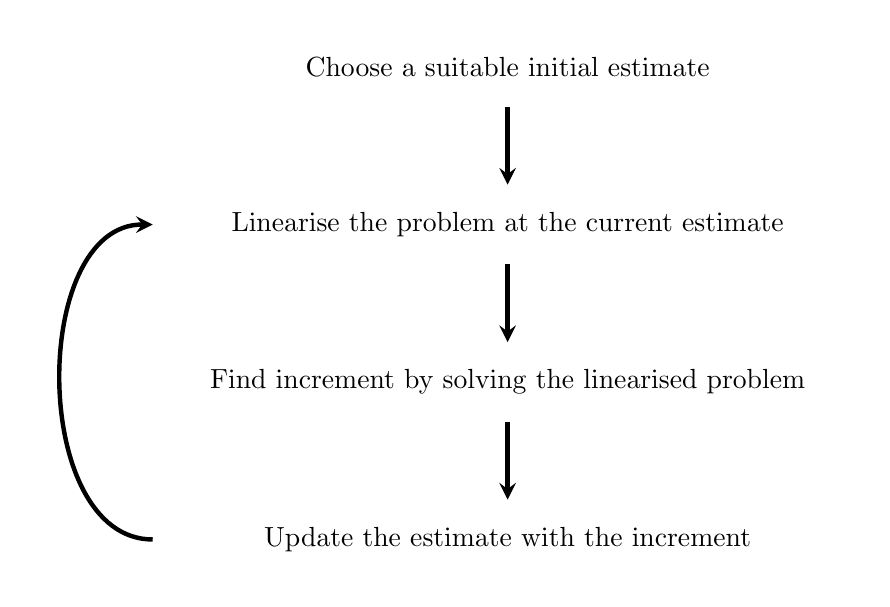
\begin{tikzpicture}[node distance=2cm]
\node (init) [process] {Choose a suitable initial estimate};
\node (linearise) [process, below of=init] {Linearise the problem at the current estimate};
\node (solve) [process, below of=linearise] {Find increment by solving the linearised problem};
\node (update) [process, below of=solve] {Update the estimate with the increment};

\draw [arrow] (init) -- (linearise);
\draw [arrow] (linearise) -- (solve);
\draw [arrow] (solve) -- (update);
\draw [arrow] (update.west) to [out=180,in=180] (linearise.west);
\end{tikzpicture}
